\chapter{Prerequisites}
\label{chapter:prerequisites}

This chapter introduces the notation used throughout the text and offers a quick overview of the
theoretical background needed in the following chapters. We shall define the classification task in
machine learning and briefly describe several machine learning algorithms heavily utilised in the
imbalanced preprocessing methods discussed in Chapter~\ref{chapter:imb-classif}. Finally, we shall
touch upon the evaluation metrics used in imbalanced classification.


\section{Notation}
\label{section:notation}

Throughout the text, we shall use the mathematical notation introduced in related books and
research literature~\cite{learning-from-imb-data, pattern-recognition}. Numbers are denoted by
lowercase letters $x, y$ or $\alpha, \beta$ and vectors are denoted by bold lowercase Roman letters
such as $\mathbf{x}, \mathbf{y}$. All vectors are column vectors; to denote a row vector, we use a
transposition operator $T$ in the superscript as $\mathbf{x}^T$. Matrices are denoted by bold
capital letters from the beginning of the alphabet, like $\mathbf{A}$ and $\mathbf{B}$.

Data samples used in machine learning for training and testing are represented as vectors, such as
$\mathbf{x}$ and $\mathbf{y}$. A dataset, a collection of data samples, is understood as a multiset
denoted by regular uppercase letters, such as $S$ or $C$. A set of labels corresponding to data
samples is denoted as $\mathcal{C}$. We use subscripts $S_{min}$ and $S_{maj}$ to denote a part of
the dataset belonging to a minority or majority class, respectively. Sometimes, a set of essential
samples to the method discussed is denoted in a different font, such as $\mathcal{N}$ or
$\mathcal{S}$.


\section{Classification}
\label{section:classification}

\emph{Classification} is one of the tasks of supervised machine learning. Classifiers try to assign
each sample $\mathbf{x}$ to a single category $y$ from a finite set of categories $\mathcal{C}$,
sometimes referred to as \emph{class labels}. Some examples of classification tasks are, for
example, assigning a genre to a book based on a brief description or flagging computer binaries as
benign or malicious. The goal of a classification task is to find a function $\mathbf{y} \colon
\mathbb{R}^d \to \mathcal{C}$ that receives a sample $\mathbf{x}$ and produces an output $y$, a
possible class label.

In the beginning, we are given a dataset holding samples $\{\mathbf{x}_1, \mathbf{x}_2,
\mathbf{x}_3, \dots, \mathbf{x}_n\}$, where each $\mathbf{x}_i$ is a d-dimensional vector living in
the euclidean vector space $\mathbb{R}^d$. Furthermore, we possess a ground truth in the form of
labels $\{y_1, y_2, y_3, \dots, y_n\}$. The domain of $y_i$ depends on the classification task. In
\emph{binary} classification, the domain is $\{0, 1\}$; in the case of classification into $k$
classes called \emph{multi-class} classification, the domain is $\{0, 1, \dots, k - 1\}$.

We usually split the provided data into \emph{training} set $\{(\mathbf{x}_i, y_i)\}_{i=1}^{m}$ and
\emph{test} set $\{(\mathbf{x}_i, y_i)\}_{i=m + 1}^{n}$. We use the training set to train a
classifier, i.e. find a function $\mathbf{y}$ that best describes the data. As our finite dataset
cannot possibly contain all possible samples $\mathbf{x}$, one of the essential requirements for a
classifier is the ability to \emph{generalise}. Generalisation is the capability to classify unseen
examples well. Once a classifier has finished training, we can evaluate its performance on unseen
data from the test set. This way, we can test how well the trained classifier generalises. We shall
discuss various evaluation metrics in Section~\ref{section:metrics}.


\section{K Nearest Neighbours - KNN}
\label{section:knn}

\emph{K Nearest Neighbours} is a non-parametric supervised machine learning algorithm. KNN can be
used for classification and regression tasks, but we shall only describe the classification
algorithm. The training part of KNN consists of storing all of the training examples smartly
because the inference uses the whole training set and is the most computationally demanding part of
the algorithm. Given a data sample $\mathbf{x} \in \mathbb{R}^d$, the algorithm finds its k-nearest
neighbours from the training set in the d-dimensional vector space. The value of k is a
hyperparameter provided by the user. Larger values of k create smoother decision boundaries and are
more resistant to noise. In comparison, smaller values of k tend to catch the training data more
precisely and may lead to overfitting. The usual metrics employed to find the k-nearest neighbours
are based on the $L_p$ norm defined as
\begin{equation}
    L_p = \left(\sum_{i=1}^{d} \lvert x_i \rvert^p\right)^{1/p}
\end{equation}
with typical values of $p$ being $ 1, 2, 3, \infty$. Once the algorithm has identified k-nearest
neighbours, classification is performed by voting. The most frequent class label among the
neighbours is assigned to the $\mathbf{x}$. There are various enhancements to KNN, such as
neighbour weighting, but we do not need to discuss them. Lastly, the nearest neighbour rule refers
to the KNN algorithm with k = 1.


\section{Support Vector Machines - SVM}
\label{section:svm}

\emph{Support Vector Machines} is a classification algorithm first proposed by
\citeauthor{svm}~\cite{svm}. It is a so-called maximum-margin classifier, as it tries to find a
decision boundary that gives the smallest generalisation error~\cite{pattern-recognition}. SVM
finds a decision boundary whose distance to the closest training example is the largest. SVM is
usually solved in the dual formulation as it is computationally easier to solve, and it allows a
reformulation using kernels~\cite{pattern-recognition}. Kernel trick is used to project data
samples to high-dimensional spaces without explicitly creating a mapping. A linear decision
boundary separating the data is found in the high-dimensional feature spaces. The authors say that
only a subset of the original data is needed to find an optimal decision boundary, and the rest of
the training data can be discarded. Vectors needed to find an optimal decision boundary are called
\emph{support vectors}.


\section{K Means}
\label{section:kmeans}

\emph{K Means} clustering algorithm is an instance of \emph{unsupervised} machine learning
algorithm. In unsupervised machine learning, we do not possess a ground truth in the form of labels
as in supervised machine learning. The goal of the K Means algorithm is to find $\mathrm{K}$
clusters $\boldsymbol{\mu}_k$ and assign each data sample to one of the clusters. The clusters and
assignments to clusters are found so that the following objective function is minimised:

\begin{equation}
    \mathrm{J} = \sum_{n=1}^N \sum_{k=1}^K r_{nk} \lVert \mathbf{x}_n - \boldsymbol{\mu}_k
    \rVert^2.
    \label{equation:k-means}
\end{equation}

Equation~\ref{equation:k-means} uses indicator variables $r_{nk} \in \{0, 1\}$ denoting whether a
sample $\mathbf{x}_n$ belongs to cluster $\boldsymbol{\mu}_k$ or not. The algorithm usually starts
by choosing initial values for clusters $\boldsymbol{\mu}_k$ randomly and continues by iterating
two steps until a stopping condition is met. The first step assigns each sample $\mathbf{x}_n$ to
the closest cluster $\boldsymbol{\mu}_k$. The second step computes new cluster centroids by
averaging the samples belonging to that cluster. Both these steps aim to minimise the objective
function $\mathrm{J}$. One drawback is that the algorithm is sensitive to the initial positions of
cluster centroids. KMeans++~\cite{kmeans++} is a possible replacement for random initialisation to
avoid poor clusterings of samples.


\section{Evaluation Metrics}
\label{section:metrics}

Having multiple evaluation metrics is extremely important when dealing with imbalanced
classification, as more often than not, a single evaluation metric does not present the whole
picture accurately. Take, for example, accuracy, the most frequently used evaluation metric in
classification. Accuracy gets biased towards the prevalent class when dealing with imbalanced
datasets~\cite{learning-from-imb-data, gosain2017, baccuracy} and, as a result, conveys unreliable
information. Imagine a dataset with 95\% of samples belonging to the negative class and the
remaining 5\% to the positive class. A classifier classifying all samples as negative would still
achieve an accuracy of 95\% and would be considered superb. Having only a single evaluation metric
would result in praising a classifier that completely ignores the positive class, which is most
often the more important one. In the following subsections, we present seven additional evaluation
metrics we shall use for reporting the results and which, when used together, usually provide more
reliable information.

We present the evaluation metrics using a \emph{confusion matrix}~\ref{table:confusion-matrix}.
The confusion matrix provides transparent information about the number of correct and incorrect
predictions in an easy-to-read table. It is essential to note that the dimensions of the matrix
depend on the number of classes we can predict. In this case, we use a $2\times2$ confusion matrix
for binary classification.  Confusion matrices divide predictions into four bins. For example,
\emph{true positives} are correctly classified positive samples; \emph{false positives} are
negative samples incorrectly classified as positive samples and so on.

\begin{table}
    \centering

    \begin{tabular}{c|cc}
        {}                 & True Positive       & True Negative       \\
        \midrule
        Predicted Positive & True Positive (TP)  & False Positive (FP) \\
        Predicted Negative & False Negative (FN) & True Negative (TN)  \\
    \end{tabular}

    \caption{\textbf{Confusion Matrix for Binary Classification.}}
    \label{table:confusion-matrix}
\end{table}

\subsection{Accuracy \& Balanced Accuracy}
\label{subsection:accuracy}

Accuracy, as we have already mentioned, is the most frequently occurring evaluation metric used in
classification. Accuracy is the fraction of the number of correctly classified samples over all
predictions and is defined, using the labels from the confusion matrix, as follows:
\begin{equation}
    \mathrm{accuracy} = \frac{TP + TN}{TP + FP + FN + TN}.
\end{equation}
Balanced accuracy~\cite{baccuracy} is defined as the arithmetic mean of accuracies in both classes:
\begin{equation}
    \mathrm{balanced\_accuracy} = \frac{1}{2}\left(\frac{TP}{TP + FN} + \frac{TN}{FP + TN}\right)
\end{equation}
Balanced accuracy provides a more reliable estimate of the classifier's performance when dealing
with imbalanced data as it prevents too optimistic estimates provided by the conventional
accuracy~\cite{baccuracy}.


\subsection{Precision, Recall \& F Score}
\label{section:precision-recall-f1}

Precision gives the percentage of samples classified as positive that actually are positive. It
measures how precise a classifier is in distinguishing true positive samples from the
rest~\cite{gosain2017}.
\begin{equation}
    \mathrm{precision} = \frac{TP}{TP + FP}
\end{equation}

Recall, sometimes called True Positive Rate, is the percentage of positive samples classified
correctly. Note that both precision and recall focus only on the class of interest, most commonly
the positive class~\cite{bad-practices}.
\begin{equation}
    \mathrm{recall} = \frac{TP}{TP + FN}
\end{equation}

Precision and Recall on their own are not sufficient to gain a good sense of the classifier's
performance~\cite{learning-from-imb-data}. $F_1$ score is a harmonic mean of Precision and Recall
and gives a fuller insight into the performance. Both Precision and Recall contribute evenly to the
final score. There exists a generalisation called the $\mathrm{F}_\beta$ score, which allows
putting more weight on either metric. The maximum possible value of $\mathrm{F_1}$ is 1, and the
lowest possible value is 0.
\begin{equation}
    \mathrm{F_1} = \frac{2 \cdot \mathrm{precision} \cdot \mathrm{recall}}{\mathrm{precision} +
    \mathrm{recall}}
\end{equation}


\subsection{Matthews Correlation Coefficient - MCC}
\label{subsection:mcc}

MCC treats true labels and predicted labels as two random variables taking on either 0 or 1 and
computes a correlation between them. Its range goes from -1 to 1, where 1 means the predictions
completely correlate with true labels, i.e. $FP = FN = 0$ and -1 means that the classifier's
prediction are always the exact opposite of the true label, i.e. $TP = TN = 0$. When the MCC
equals 0, the classifier's predictions are as good as a flip of a coin. MCC, as opposed to the
previous metrics uses all entries in the confusion matrix and is also resistant to class imbalance.
\begin{equation}
    \mathrm{MCC} = \frac{TN \cdot TP - FN \cdot FP}{\sqrt{(TP + FP)(TP + FN)(TN + FP)(TN + FN)}}
\end{equation}


\subsection{Precision Recall Curve - PR}

Up until now, all evaluation metrics gave only a single number evaluating the classifier's
performance. Precision Recall Curve, unlike previous methods, plots Precision and Recall values at
many different decision thresholds, as shown in Figure~\ref{figure:pr-curve}. A classifier's
performance can be assessed by computing the area under the curve. The best performance is obtained
at a point $(1.0, 1.0)$ where both Precision and Recall reach their maximum values.

\begin{figure}
    \centering
    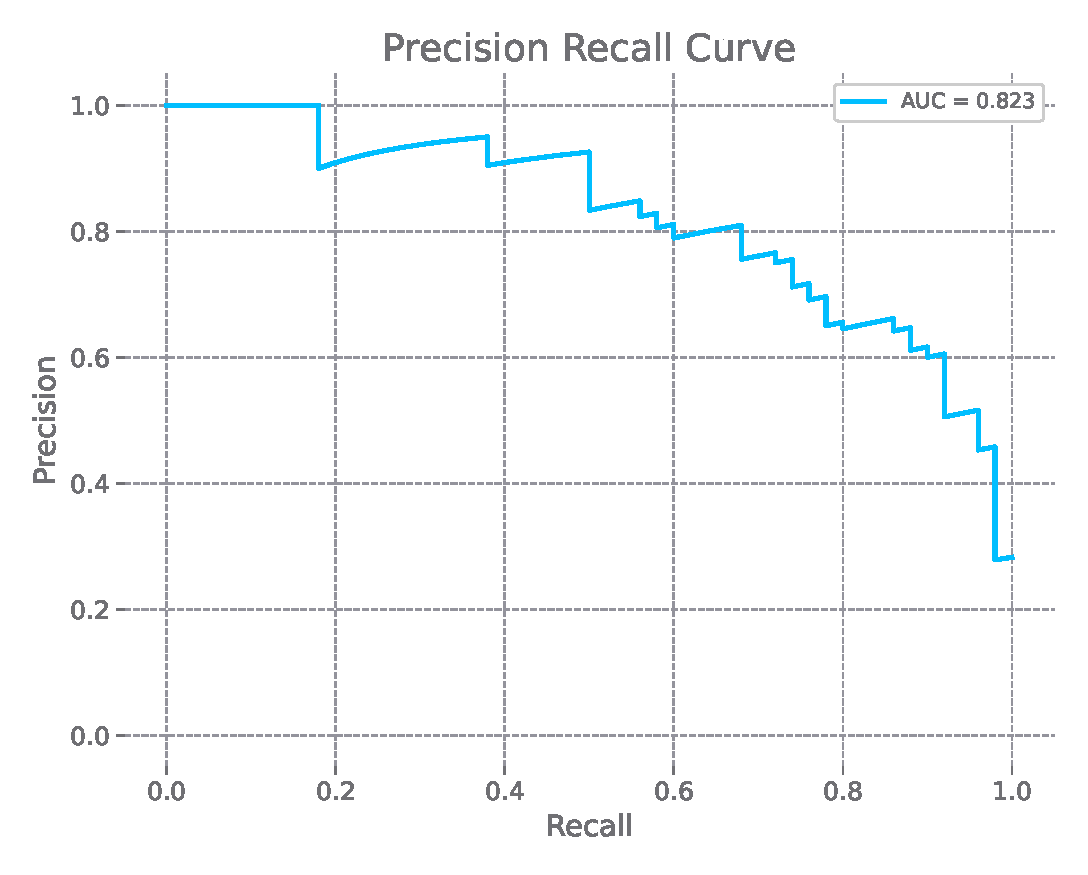
\includegraphics[width=0.75\linewidth]{figures/pr_curve.eps}
    \caption{
        \textbf{Precision Recall Curve.} The legend shows the value of the area under the curve.
    }
    \label{figure:pr-curve}
\end{figure}


\subsection{Receiver Operating Characteristic Curve - ROC}
\label{subsection:roc}

The most important metric for us is the ROC Curve. ROC Curve plots False Positive Rate, $FPR =
\frac{FP}{FP + TN}$, on the horizontal axis against True Positive Rate, $TPR = \frac{TP}{TP + FN}$,
on the vertical axis, computed at several decision thresholds, as shown in
Figure~\ref{figure:roc-curve}. Again, a single number giving the performance of a classifier can be
obtained by computing the are under the curve. As FPR and TPR go against each other, the perfect
classification performance is obtained at a point $(0, 1)$. ROC Curve, as MCC, is also resistant to
class imbalance.

\begin{figure}
    \centering
    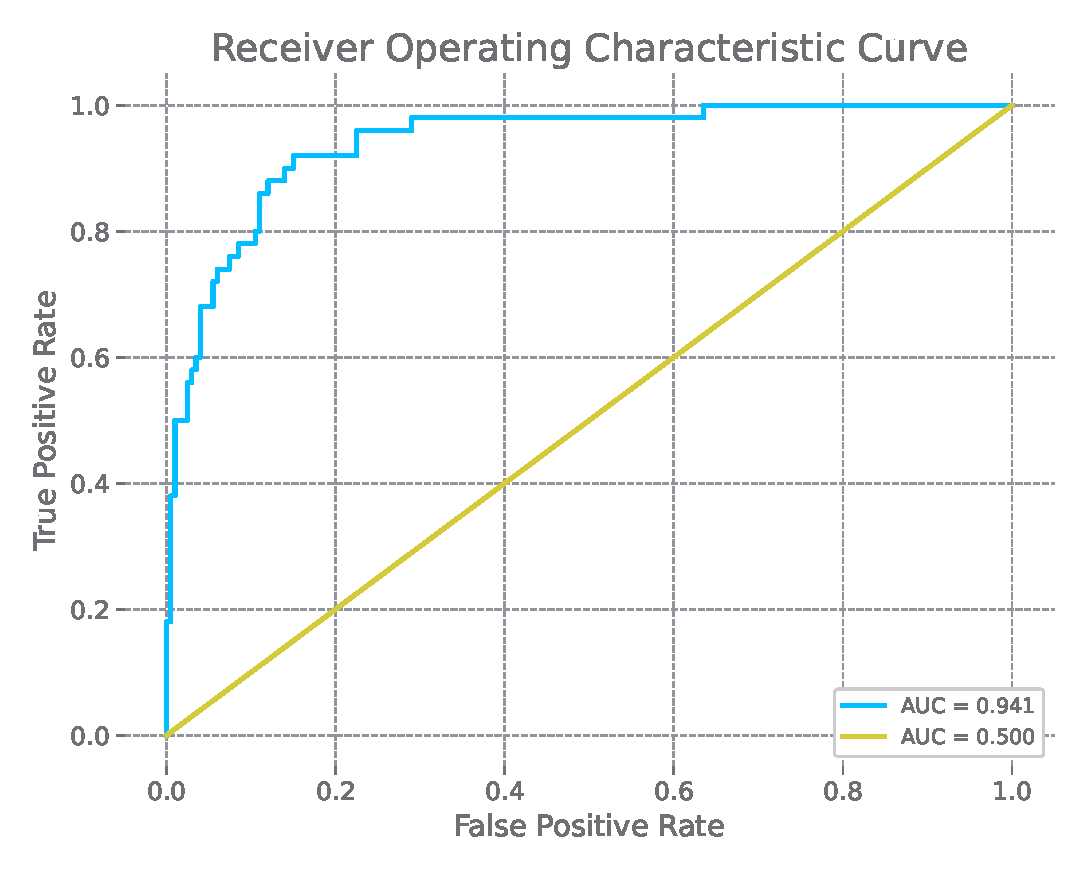
\includegraphics[width=0.75\linewidth]{figures/roc_curve.eps}
    \caption{
        \textbf{Receiver Operating Characteristic Curve} The legend shows the value of the area
        under the curves. The blue curve belongs to a Logistic Regression classifier, and the
        yellow curve belongs to the dummy classifier performing random predictions.
    }
    \label{figure:roc-curve}
\end{figure}
